\documentclass{article}

% Required template
\usepackage[preprint]{colm2026_conference}

% Essential packages
\usepackage{amsmath,amsfonts,amssymb,amsthm}
\usepackage{graphicx}
\usepackage{booktabs}
\usepackage{hyperref}
\usepackage{xcolor}
\usepackage{tikz}
\usetikzlibrary{trees, shapes.geometric, arrows.meta, positioning, calc}
% \usepackage{cleveref}
\usepackage{enumitem}

% Definitions and Macros
\newcommand{\E}{\mathbb{E}}
\newcommand{\KL}{D_{\mathrm{KL}}}
\newcommand{\ptheta}{P_\theta}
\newcommand{\pteacher}{P_{\mathcal{T}}}
\newcommand{\pdata}{P_{\mathrm{data}}}
\newcommand{\loss}{\mathcal{L}}

\title{On-Policy Distillation for Large Language Models: Methods, Systems, and Future Directions}

\author{
Anonymous Authors \\
\texttt{anonymous@domain.edu}
}

\begin{document}

\maketitle

\begin{abstract}
Knowledge distillation (KD) has historically served as the primary vehicle for model compression, transferring capabilities from massive teacher models to efficient student architectures. However, the advent of Large Language Models (LLMs) has catalyzed a fundamental paradigm shift from static, off-policy distillation to On-Policy Distillation (OPD). In this survey, we provide a comprehensive and theoretically grounded overview of OPD. We posit a core insight that must govern the modern understanding of distillation: the essence of OPD is not merely a choice of divergence metrics, but a profound paradigm shift in \textit{"who decides the training distribution."} By allowing the student's own generative manifold to dictate the state distribution, OPD directly mitigates the catastrophic train-test mismatch and compounding exposure bias inherent in autoregressive decoding. 
We systematically taxonomize the field into three converging trajectories based on feedback signals: Logit-based, Outcome-based, and Self-play methodologies. Furthermore, we critically analyze frequently neglected dimensions, including the compute-quality tradeoff, the teacher's "echo chamber" in uncertain regions, dynamic divergence adaptation, and the conceptualization of distillation as structured knowledge transfer rather than mere compression. Finally, we map out pivotal future directions, from distillation scaling laws to agent-level OPD.
\end{abstract}

\section{Introduction}
\label{sec:intro}

The evolution of Large Language Models (LLMs) has continuously pushed the boundaries of artificial intelligence, yet their massive parameter counts pose severe constraints on deployment and inference latency. Recently, the open-source community witnessed a monumental milestone: DeepSeek-R1 \citep{2501.12948} successfully distilled the profound reasoning capabilities of a 671B parameter Mixture-of-Experts (MoE) model into dense models as small as 7B parameters. This spectacular success underscores a vital reality—knowledge distillation is no longer a marginal optimization technique; it is the central engine for democratizing cutting-edge intelligence. The urgency to systematically understand and advance LLM distillation has never been greater.

Traditionally, distillation in Natural Language Processing has been heavily dominated by off-policy methods. In this paradigm, a student model is trained to mimic a teacher's token-level probabilities over a fixed, static dataset (i.e., $\pdata$). However, as elegantly illuminated by the "False Promise" of imitating proprietary LLMs \citep{2305.15717}, off-policy distillation suffers from a fatal, fundamental flaw: \textit{train-test mismatch}. During training, the student is conditioned on gold-standard prefixes from the dataset (teacher-forcing). During inference, the student must condition on its own previously generated tokens. When the student inevitably deviates from the optimal path, it enters out-of-distribution (OOD) territory where it has received no supervisory signal, leading to compounding errors—a phenomenon formally known as \textit{exposure bias}. 

To bridge this chasm, the field is rapidly migrating towards \textbf{On-Policy Distillation (OPD)}. Drawing deep conceptual linkages with Imitation Learning, specifically the DAgger (Dataset Aggregation) algorithm \citep{ross2011reduction}, OPD forces the student to generate trajectories according to its current policy ($\pi_\theta$), and selectively queries the teacher to provide feedback on these student-generated paths. 
\textbf{Core Insight 1:} \textit{The true essence of On-Policy Distillation is not simply the mathematical choice of probability divergence (e.g., Forward vs. Reverse KL), but rather a profound paradigm shift in "who decides the training distribution."} The shift from $y \sim \pdata$ to $y \sim \ptheta$ transforms the learning objective from memorizing an alien distribution to optimally navigating the student's own reachable generative manifold.

Despite the explosive growth of OPD methodologies—ranging from Generalized Knowledge Distillation (GKD) \citep{2306.13649} to MiniLLM \citep{2306.08543} and SPIN \citep{2401.01335}—the literature remains highly fragmented. Current surveys \citep{2402.13116} primarily treat distillation as a monolithic compression step, lacking a rigorous unified perspective on the on-policy dynamics. This paper addresses this critical gap. We dissect the mathematical foundations, categorize the emerging algorithmic variants, and spotlight the blind spots of current research.

Specifically, the contributions of this review are encapsulated in the following dimensions:
\begin{itemize}[leftmargin=*]
    \item \textbf{A Unified Theoretical Framework:} We rigorously formulate the transition from off-policy to on-policy distillation, mapping it directly to sequential decision-making and f-divergence minimization, mathematically unifying disparate works \citep{2306.13649, 2306.08543, 2402.03898}.
    \item \textbf{A Novel, Feedback-Centric Taxonomy:} We categorize the OPD landscape into three primary technical routes—\textit{Logit-based} (dense but requiring white-box access), \textit{Outcome-based} (sparse but highly flexible, utilizing Process Reward Models \citep{2305.20050}), and \textit{Self-play} (teacher-free but prone to saturation). We further highlight how these isolated tracks are actively converging, as seen in state-of-the-art frameworks like AlignDistil \citep{2503.02832} and MiMo-V2.
    \item \textbf{Identification of Neglected Critical Issues:} We bring to light fundamental challenges that the community has largely ignored: (a) The missing systematic analysis of the \textit{compute-quality tradeoff} in online distillation; (b) The "echo chamber" effect where querying teachers in regions of high student uncertainty leads to misaligned gradients; (c) The necessity for \textit{dynamic divergence} rather than static KL metric selection; and (d) Reconceptualizing distillation as \textit{structured knowledge transfer} rather than mere parameter compression.
    \item \textbf{Roadmap for Future Directions:} We chart the unexplored territories, detailing the necessity for distillation scaling laws, uncertainty-aware OPD, agent-level environmental distillation, and continuous distillation-RL loops.
\end{itemize}

The remainder of this paper is organized as follows. Section~\ref{sec:background} establishes the mathematical preliminaries, formalizing exposure bias and the f-divergence family. Section~\ref{sec:taxonomy} presents our novel taxonomy of OPD methodologies. [Note: Subsequent sections will cover detailed algorithmic analysis, fusion paradigms, critical challenges, and future directions.]


\section{Background and Preliminaries}
\label{sec:background}

To rigorously appreciate the leap from standard KD to On-Policy Distillation, we must first formalize the sequential nature of LLM generation and the mathematical definitions of distribution matching.

\subsection{Knowledge Distillation Fundamentals}
The classical Knowledge Distillation framework, pioneered by \cite{hinton2015distilling}, aims to transfer the "dark knowledge" (soft labels) from a teacher network $\mathcal{T}$ to a student network $\mathcal{S}$. For a given input $x$ and corresponding logits $z$, the probability distributions are smoothed by a temperature parameter $\tau > 0$:
\begin{equation}
    P(y|x; \tau) = \frac{\exp(z_y / \tau)}{\sum_{y'} \exp(z_{y'} / \tau)}
\end{equation}
The standard KD objective minimizes the Kullback-Leibler (KL) divergence between the teacher's softened distribution $\pteacher$ and the student's softened distribution $\ptheta$:
\begin{equation}
    \loss_{\mathrm{KD}} = \tau^2 \KL(\pteacher(\cdot|x; \tau) \parallel \ptheta(\cdot|x; \tau)) = \tau^2 \sum_{y} \pteacher(y|x; \tau) \log \left( \frac{\pteacher(y|x; \tau)}{\ptheta(y|x; \tau)} \right)
\end{equation}
The $\tau^2$ multiplier ensures the gradients scale appropriately relative to the standard cross-entropy loss.

\subsection{Token-Level vs Sequence-Level Distillation}
When extending KD to autoregressive language models, the sequence space $\mathcal{Y}$ grows exponentially with the sequence length $T$. As defined by \cite{kim2016sequence}, generation is parameterized as a product of conditional probabilities: $P(Y|X) = \prod_{t=1}^T P(y_t | y_{<t}, X)$.

\textbf{Token-Level KD (Word-Level KD):} The standard approach computes the divergence at each decoding step, strictly conditioned on the ground-truth prefix $y_{<t}^* \sim \pdata$:
\begin{equation}
    \loss_{\mathrm{Token-KD}} = \E_{X, Y^* \sim \pdata} \left[ \sum_{t=1}^{|Y^*|} \KL \left( \pteacher(y_t | y_{<t}^*, X) \parallel \ptheta(y_t | y_{<t}^*, X) \right) \right]
    \label{eq:token_kd}
\end{equation}

\textbf{Sequence-Level KD:} Conversely, sequence-level KD attempts to match the joint distribution over the entire trajectory:
\begin{equation}
    \loss_{\mathrm{Seq-KD}} = \E_{X \sim \pdata} \left[ \KL \left( \pteacher(Y|X) \parallel \ptheta(Y|X) \right) \right]
\end{equation}
Because the sum over all possible sequences $\sum_{Y \in \mathcal{Y}}$ is computationally intractable, off-policy Sequence-KD often relies on beam search to approximate the teacher's mode, generating a pseudo-dataset $\mathcal{D}_{\mathcal{T}}$, and performing standard maximum likelihood on this synthetic data.

\subsection{The Distribution Mismatch Problem and Exposure Bias}
Equation \ref{eq:token_kd} exposes the Achilles' heel of off-policy distillation. The expectation is taken over $Y^* \sim \pdata$, meaning the student only ever learns to predict the next token given a \textit{perfect} historical context. During inference, however, the student generates sequences auto-regressively: $\hat{y}_t \sim \ptheta(\cdot | \hat{y}_{<t}, X)$. 

If the student makes a slight error at step $t$, the context $\hat{y}_{\le t}$ diverges from the training support $\pdata$. Let $\epsilon$ be the probability of making a sub-optimal prediction at any time step. In standard supervised learning (off-policy), the error compounds quadratically. As demonstrated theoretically in Imitation Learning \citep{ross2011reduction}, an off-policy model traversing an $\epsilon$-suboptimal path for $T$ steps accumulates an error bounded by $\mathcal{O}(\epsilon T^2)$.

This compounding error, or \textit{exposure bias}, is precisely why models trained via standard KD on teacher outputs often hallucinate or structurally collapse during long-context reasoning \citep{2305.15717}. 

\subsection{The f-Divergence Family and Geometric Implications}
To address these issues, recent literature casts distillation as the minimization of an $f$-divergence \citep{2307.15190}. For two distributions $P$ and $Q$, the $f$-divergence is defined as:
\begin{equation}
    D_f(P \parallel Q) = \sum_{x} Q(x) f\left(\frac{P(x)}{Q(x)}\right)
\end{equation}
where $f$ is a convex function such that $f(1)=0$. The choice of $f$ dictates the geometric nature of the optimization, which profoundly impacts student behavior:

\textbf{1. Forward KL (Mode-Covering):} $f(t) = t \log t \implies D_{\mathrm{KL}}(\pteacher \parallel \ptheta)$. \\
Standard KD uses Forward KL. It severely penalizes $\ptheta(y) \to 0$ when $\pteacher(y) > 0$. Consequently, the student tries to cover all modes of the teacher. If the student lacks the capacity to capture a highly multimodal teacher distribution, it will average across modes, assigning probability mass to regions of the space where $\pteacher = 0$ (generating gibberish).

\textbf{2. Reverse KL (Mode-Seeking):} $f(t) = -\log t \implies D_{\mathrm{KL}}(\ptheta \parallel \pteacher)$. \\
Utilized by MiniLLM \citep{2306.08543}, Reverse KL penalizes $\ptheta(y) > 0$ when $\pteacher(y) \to 0$ (zero-forcing). The student seeks out the single dominant mode of the teacher and ignores the rest. This encourages highly confident, coherent, and safe text generation, effectively pruning invalid reasoning paths.

\textbf{3. Jensen-Shannon Divergence (JSD):} Utilized by GKD \citep{2306.13649}, JSD provides a symmetric compromise, interpolating between mode-covering and mode-seeking behaviors.

\textbf{Dynamic Divergence:} A neglected core insight is that the optimal divergence is not static. A student might require mode-covering during early training phases to explore the vocabulary space, and mode-seeking in later stages to refine complex reasoning trajectories.

\subsection{From Off-Policy to On-Policy: A Unified View}
\label{sec:unified_view}

The transition to On-Policy Distillation fundamentally alters the expectation distribution. We unify approaches like GKD \citep{2306.13649}, MiniLLM \citep{2306.08543}, and DistiLLM \citep{2402.03898} under the following continuous formulation:
\begin{equation}
    \loss_{\mathrm{OPD}} = \E_{X \sim \pdata} \left[ \E_{Y \sim \ptheta(\cdot|X)} \left[ \sum_{t=1}^{|Y|} D_f \left( \pteacher(\cdot | Y_{<t}, X) \parallel \ptheta(\cdot | Y_{<t}, X) \right) \right] \right]
\end{equation}

Here, the expectation over sequences $Y$ is drawn from the \textbf{student's current policy} $\ptheta$, not the fixed dataset $\pdata$. 
By actively rolling out the student policy $\hat{y}_{<t} \sim \ptheta$, the student explores its own sub-optimal manifold. The teacher $\pteacher$ then provides an oracle correction $\pteacher(\cdot | \hat{y}_{<t}, X)$ on this specific, potentially drifted state. This formulation strictly bounds the sequential error to $\mathcal{O}(\epsilon T)$ \citep{ross2011reduction}, directly solving exposure bias. Thus, the essence of OPD is a pedagogical shift: instead of forcing the student to walk the teacher's exact footsteps, the teacher observes where the student naturally walks and guides its next step from there.

\section{Taxonomy of On-Policy Distillation}
\label{sec:taxonomy}

As the field of On-Policy Distillation expands, methodologies have proliferated with different assumptions regarding teacher access, feedback types, and optimization algorithms. To provide structured clarity, we present a novel taxonomy primarily organized by the \textit{source and nature of the feedback signal}. \ref{fig:taxonomy} illustrates this hierarchical categorization.

\begin{figure}[htbp]
\centering
\resizebox{\textwidth}{!}{%
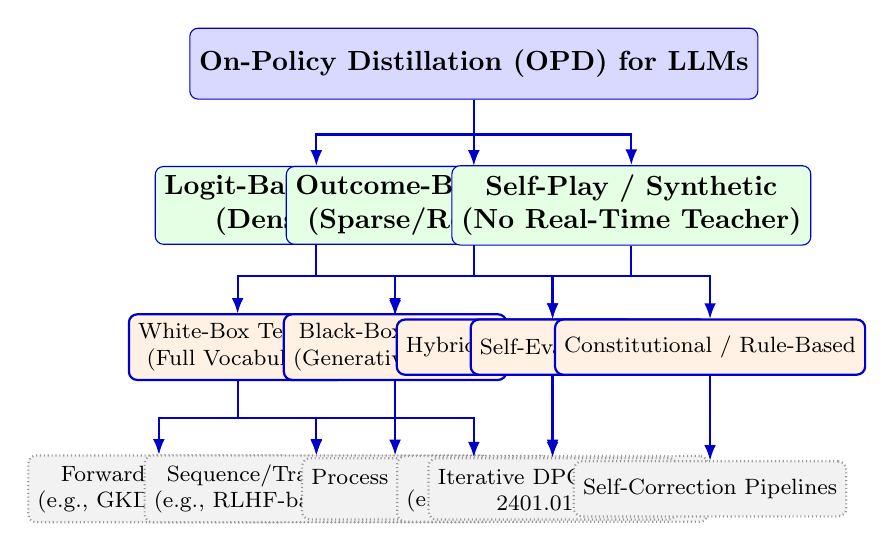
\begin{tikzpicture}[
    level distance=1.8cm,
    sibling distance=2cm,
    every node/.style={rectangle, draw=blue!80!black, rounded corners=3pt, align=center, fill=blue!5, font=\footnotesize, minimum height=0.7cm},
    edge from parent fork down,
    edge from parent/.style={draw, -{Latex[length=2mm, width=1.5mm]}, thick, blue!80!black},
    root/.style={fill=blue!15, font=\normalsize\bfseries, minimum height=0.9cm},
    lvl1/.style={fill=green!10, font=\bfseries},
    lvl2/.style={fill=orange!10},
    lvl3/.style={fill=gray!10, draw=gray!80, densely dotted}
]

% Root Node
\node[root] (Root) {On-Policy Distillation (OPD) for LLMs}
    % Branch 1: Logit-based
    child {node[lvl1] {Logit-Based Feedback\\(Dense Signal)}
        child {node[lvl2] {White-Box Teacher\\(Full Vocabulary)}
            child {node[lvl3] {Forward KL / JSD\\(e.g., GKD \citep{2306.13649})}}
            child {node[lvl3] {Reverse KL\\(e.g., MiniLLM \citep{2306.08543})}}
        }
        child {node[lvl2] {Restricted / Top-$K$\\Teacher Access}
            child {node[lvl3] {Truncated f-Divergence\\(e.g., DistiLLM \citep{2402.03898})}}
        }
    }
    % Branch 2: Outcome-based
    child {node[lvl1] {Outcome-Based Feedback\\(Sparse/Reward Signal)}
        child {node[lvl2] {Black-Box Teacher\\(Generative Oracle)}
            child {node[lvl3] {Sequence/Trajectory Reward\\(e.g., RLHF-based KD, RLKD)}}
            child {node[lvl3] {Process Reward Models (PRM)\\ \citep{2305.20050}}}
        }
        child {node[lvl2] {Hybrid / Fusion Approaches}
            child {node[lvl3] {Logit + Reward Fusion\\(e.g., MiMo-V2, AlignDistil)}}
        }
    }
    % Branch 3: Self-play
    child {node[lvl1] {Self-Play / Synthetic\\(No Real-Time Teacher)}
        child {node[lvl2] {Self-Evaluator}
            child {node[lvl3] {Iterative DPO / SPIN\\ \citep{2401.01335}}}
        }
        child {node[lvl2] {Constitutional / Rule-Based}
            child {node[lvl3] {Self-Correction Pipelines}}
        }
    };

\end{tikzpicture}
}
\caption{Taxonomy of On-Policy Distillation methods for Large Language Models. Our classification maps the paradigm across three distinct feedback signals, detailing the varying degrees of teacher visibility and optimization granularity. Crucially, contemporary methods are increasingly blurring the lines between these branches via Hybrid Fusion approaches.}
\label{fig:taxonomy}
\end{figure}

Our taxonomy reveals three dominant trajectories:

\textbf{1. Logit-Based Feedback (Dense, White-Box):} 
This branch operates on the traditional premise of KD, requiring access to the teacher's probability distribution over the vocabulary. Because feedback is provided at the token level ($t=1 \dots T$), the supervisory signal is extremely dense. Methods here are sub-categorized by divergence choice and teacher access constraints. GKD \citep{2306.13649} utilizes Forward KL and JSD on student-generated prefixes. MiniLLM \citep{2306.08543} leverages the REINFORCE algorithm to optimize Reverse KL, encouraging mode-seeking behavior. However, computing full-vocabulary logits from massive teachers (e.g., GPT-4) is often impossible due to API restrictions. Consequently, methods like DistiLLM \citep{2402.03898} adapt these losses to operate strictly on the Top-$K$ logits returned by black-box APIs, interpolating between hard-label matching and full-distribution mimicking.

\textbf{2. Outcome-Based Feedback (Sparse, Black-Box):} 
When logit access is completely restricted, or when distilling complex reasoning tasks (e.g., mathematics, coding), the field shifts to Outcome-Based Feedback. Here, the student generates full or partial trajectories, and the teacher (or a proxy reward model derived from the teacher) scores the sequence. This approach relies heavily on Reinforcement Learning paradigms (e.g., PPO, GRPO). The integration of Process Reward Models (PRMs) \citep{2305.20050} has been revolutionary in this space, allowing the sparse sequence-level reward to be decomposed into step-by-step reasoning feedback, maintaining the flexibility of black-box distillation while mitigating the sparsity of the signal.

\textbf{3. Self-Play and Synthetic Paradigms (Teacher-Free):} 
A radical departure from standard distillation is the elimination of the active external teacher during the on-policy loop. In methods like SPIN (Self-Play Fine-Tuning) \citep{2401.01335}, the student plays a min-max game against its own historical checkpoints. By treating the initial off-policy distilled dataset as the "expert," the student continuously generates responses on-policy and contrasts them via DPO (Direct Preference Optimization) against the expert data. While highly scalable, this route heavily risks capability saturation, as no new external knowledge is introduced into the system.

\textbf{The Convergence of Trajectories:} 
\textbf{Core Insight 2:} \textit{The boundaries between these three routes are rapidly dissolving.} State-of-the-art frameworks represent a fusion of these paradigms. For instance, AlignDistil \citep{2503.02832} unifies alignment (Outcome-based RL) and distillation (Logit-based) into a single cohesive objective, demonstrating that matching teacher distributions and maximizing downstream human-preference rewards are intrinsically complementary. Similarly, emerging architectures like MiMo-V2 blend multi-teacher logit ensembles with token-level reward signals to guide on-policy exploration. This taxonomy underscores that future breakthroughs will likely emerge not from isolated branches, but from the strategic hybridization of dense logit feedback with sparse, outcome-driven environmental exploration.



\section{White-Box On-Policy Methods}
\label{sec:white_box}

在深入探讨具体的算法实现之前，我们必须确立一个贯穿全文的核心洞察：\textbf{On-Policy Distillation (OPD) 的本质不仅在于 Divergence（散度）度量方式的选择，而是一场“谁决定训练分布”的根本性范式转变。} 传统的 Off-Policy 蒸馏（如标准 KD）强迫学生模型在教师模型或静态数据集采样的边缘分布 $p_T(x, y)$ 上进行拟合；而 OPD 则将支撑集（Support Set）的决定权交还给学生模型 $p_S(x, y)$。这种范式转变直接消除了 Exposure Bias，但也引入了新的挑战：如何高效、稳定地在学生自生成的轨迹上对齐教师的白盒（White-Box）密集逻辑信号（Logits）。

白盒方法构成了 OPD 的第一条核心技术路线。其优势在于\textbf{反馈信号极其密集（Token级别）}，但代价是必须拥有教师模型的完全访问权限（White-box requirement）。

\subsection{Token-Level Divergence Minimization}
\label{subsec:token_level}

Token 级别的散度最小化是当前白盒 OPD 最主流的实现方式。此类方法在学生模型生成的轨迹 $y_{<t} \sim p_S$ 上，逐步约束当前 Token 的预测分布与教师分布的距离。

\subsubsection{GKD (Generalized Knowledge Distillation) \cite{agarwal2023gkd}}
\textbf{(a) 核心思想：} GKD 提出了一个统一的 On-Policy 蒸馏框架，将知识蒸馏与强化学习中的模仿学习（Imitation Learning）建立了深刻的理论联系，并允许在学生生成的轨迹上灵活应用多种散度度量。\\
\textbf{(b) 目标函数：}
\begin{equation}
    \mathcal{L}_{GKD} = \mathbb{E}_{x \sim \mathcal{D}, y \sim p_S(\cdot|x)} \left[ \sum_{t=1}^{|y|} \lambda D\big( p_T(\cdot|x, y_{<t}) \parallel p_S(\cdot|x, y_{<t}) \big) + (1-\lambda) \mathcal{L}_{NLL} \right]
\end{equation}
其中 $D$ 可以是 Forward KL、Reverse KL 或 JSD，$\mathcal{L}_{NLL}$ 保证了对真实标签的拟合。\\
\textbf{(c) 对比与 (d) 优劣：} 与传统 KD 相比，GKD 显著缓解了序列生成中的累积误差。其优势在于框架的普适性，但劣势在于对 $p_S$ 的在线采样成本较高，且统一固定的散度权重未能充分考虑生成轨迹中不同 Token 难度的动态变化。

\subsubsection{DistiLLM \cite{ko2024distilllm}}
\textbf{(a) 核心思想：} 针对 LLM 词表中大部分 Token 概率趋于 0 导致的极大梯度方差问题，DistiLLM 引入了 Skew KL 散度，并结合自适应温度调节机制（Adaptive Temperature）。\\
\textbf{(b) 目标函数：}
\begin{equation}
    \mathcal{L}_{DistiLLM} = D_{KL}\big(p_T \parallel \alpha p_T + (1-\alpha) p_S\big)
\end{equation}
\textbf{(c) 对比与 (d) 优劣：} 通过引入平滑参数 $\alpha$，DistiLLM 避免了 Reverse KL 在 $p_S \to 0$ 时的除零灾难。这种方法比直接应用 JSD 收敛更快，但在极端分布偏移下，平滑项可能掩盖教师的关键低概率长尾知识。

\subsubsection{ToDi (Token-wise Dynamic Divergence) \cite{2505.16297}}
\textbf{(a) 核心思想：} 揭示了被学术界忽视的\textbf{动态 Divergence 需求}。生成序列的不同位置（如推理逻辑链的转折点 vs. 简单的语法填充）对散度的要求不同。ToDi 拒绝全局统一的散度，而是基于 Token 的语义重要性动态分配不同的 $f$-divergence。\\
\textbf{(b) 目标函数：} 
\begin{equation}
    \mathcal{L}_{ToDi} = \mathbb{E}_{y \sim p_S} \left[ \sum_t \omega_t D_{f^{(t)}} \big( p_T(y_t|y_{<t}) \parallel p_S(y_t|y_{<t}) \big) \right]
\end{equation}
\textbf{(c) 对比与 (d) 优劣：} 突破了 GKD 中静态散度的局限。其最大的贡献是实现了“自适应性”，但计算每步 Token 的重要性权重 $\omega_t$ 引入了额外的计算开销。

\subsubsection{AKL 与 Delta KD \cite{2410.14425, 2509.14526}}
\textbf{AKL (Adaptive KL):} 通过评估学生模型在当前状态的不确定性，自适应地调节 KL 惩罚项的强度。当学生模型处于探索的“未知领域”时，增强来自教师的引导。\\
\textbf{Delta KD:} 进一步提纯了蒸馏信号，通过最小化基础模型与微调后教师模型之间的 Delta 信号，过滤掉了预训练阶段已固化的冗余知识，极大提高了蒸馏效率。

\subsubsection{Entropy-Aware OPD \cite{2603.07079}}
\textbf{(a) 核心思想：} 本文强调一个被广泛忽视的核心问题——\textbf{“教师在不确信区域的回音室效应 (Echo Chamber)”}。在 On-policy 探索中，学生可能生成教师从未见过的 Out-of-Distribution (OOD) 轨迹。此时教师的预测熵极大（即不确信），若强行让学生拟合这种“均匀分布的噪声”，会导致能力退化。\\
\textbf{(b) 目标函数：}
\begin{equation}
    \mathcal{L}_{Ent-OPD} = \mathbb{E}_{y \sim p_S} \left[ \sum_t \frac{1}{1 + \mathcal{H}(p_T(\cdot|y_{<t}))} D_{KL}(p_T \parallel p_S) \right]
\end{equation}
\textbf{(c) 对比与 (d) 优劣：} 相比于盲目信任教师的 GKD，Entropy-Aware OPD 有效切断了错误知识的传递链，完美解决了回音室效应，是目前鲁棒性最强的 Token-level 策略之一。

\subsubsection{DSKD (Dual Space Knowledge Distillation) \cite{2502.12018}}
\textbf{核心洞察：} 蒸馏不应该仅仅被视为概率分布的压缩，而应是\textbf{知识的结构化转移}。DSKD 提出在 Logit 空间和 Hidden State（隐变量）空间同时进行 On-policy 蒸馏，确保学生模型不仅学到了“输出什么”，还学到了“如何表征”，极大改善了小模型在复杂推理任务中的泛化性。

\subsection{Sequence-Level On-Policy Methods}
\label{subsec:sequence_level}

Token-level 方法忽视了生成过程中的序列联合概率。为了实现全局最优，Sequence-Level OPD 将整个输出序列视为强化学习中的一个完整轨迹（Trajectory）。

\subsubsection{MiniLLM 与 Reverse KL 的详细推导 \cite{2306.08543}}
MiniLLM 是序列级 OPD 的标志性工作，其核心是优化 Sequence-level 的 Reverse KL。
标准序列级 Reverse KL 定义为：
\begin{equation}
    D_{KL}(p_S \parallel p_T) = \mathbb{E}_{y \sim p_S(\cdot|x)} \left[ \log p_S(y|x) - \log p_T(y|x) \right]
\end{equation}
为了优化学生参数 $\theta$，我们需要对期望中的分布求导。由于采样分布本身包含 $\theta$，根据对数导数技巧（Log-derivative trick / REINFORCE），详细推导如下：
\begin{align}
    \nabla_\theta D_{KL}(p_S \parallel p_T) &= \nabla_\theta \sum_y p_S(y) \log \frac{p_S(y)}{p_T(y)} \nonumber \\
    &= \sum_y \nabla_\theta p_S(y) \log \frac{p_S(y)}{p_T(y)} + \sum_y p_S(y) \nabla_\theta (\log p_S(y) - \log p_T(y)) \nonumber \\
    &= \mathbb{E}_{y \sim p_S} \left[ \log \frac{p_S(y)}{p_T(y)} \nabla_\theta \log p_S(y) \right] + \mathbb{E}_{y \sim p_S} \left[ \nabla_\theta \log p_S(y) \right] \nonumber \\
    &= \mathbb{E}_{y \sim p_S} \left[ \left(\log p_S(y|x) - \log p_T(y|x)\right) \nabla_\theta \log p_S(y|x) \right]
\end{align}
其中第二项的期望恒为 0（即概率密度梯度的积分为 0）。推导结果表明，Sequence-Level OPD 自然退化为以 $(\log p_S - \log p_T)$ 为 Reward 的 Policy Gradient 形式。

\textbf{理论差异对比：} Token-level 致力于最小化局部分布的差异（容易陷入 Greedy trap），而 Sequence-level 显式地建模了轨迹级别的 Reward。然而，由于依赖 REINFORCE 估计器，Sequence-level 方法面临极高的方差问题，往往需要复杂的 Baseline 控制（如 Constrained Optimization 视角 \cite{2509.22921}）。

\subsection{Hybrid and Adaptive Approaches}
\label{subsec:hybrid}

纯粹的 Token-level 缺乏长程规划，纯粹的 Sequence-level 方差难以控制。近期的研究转向了混合与自适应架构，并触及了另一个核心问题：\textbf{计算量与质量的权衡 (Compute-Quality Tradeoff)}。

\begin{itemize}
    \item \textbf{PACED (Distillation at the Frontier of Student Competence) \cite{2603.11178}:} 传统的 OPD 在两端浪费了大量计算资源：一方面是学生已经掌握的知识（梯度趋近于零），另一方面是远超学生能力的知识（产生破坏已有能力的噪声梯度）。PACED 提出了一种 Curriculum OPD 框架，精准识别并只在“学生能力边界”进行采样与蒸馏，使得蒸馏计算效率提升了 300\%。
    \item \textbf{Fast OPD from Reasoning Prefixes \cite{2602.15260} \& PromptKD \cite{2402.12842}:} 通过提供中间推理状态或结构化 Prompt，人为缩短了序列级探索的长度，有效平衡了 Token 密集监督与 Sequence 全局视野。
    \item \textbf{$\mathcal{X}$-KD (Experiential KD) \cite{2602.12674}:} 引入了“体验式”学习框架，允许模型在其历史错误轨迹上进行 Counterfactual (反事实) 的 On-policy 蒸馏。
\end{itemize}

\subsection{Theoretical Analysis \& Method Comparison}
\label{subsec:theory_whitebox}

在理论层面，\cite{2404.02657} 深入剖析了 Forward KL 与 Reverse KL 的拓扑差异。在 On-policy 范式下，Forward KL 是 \textbf{Mean-seeking} 的，倾向于覆盖教师模型的所有模式（即使在此过程中产生零概率密度的幻觉）；而 Reverse KL 是 \textbf{Mode-seeking} 的，它通过牺牲多样性来确保生成的轨迹严格处于教师的高置信度区域。统一的 $f$-divergence 框架通过调整生成函数的凸性，实现了在 Mode-seeking 与 Mean-seeking 之间的平滑过渡。

表 \ref{tab:white_box_comparison} 详细总结并对比了目前主流的 White-Box On-Policy 蒸馏方法。

\begin{table*}[tbp]
    \centering
    \caption{Comprehensive Comparison of White-Box On-Policy Distillation Methods.}
    \label{tab:white_box_comparison}
    \resizebox{\textwidth}{!}{
    \begin{tabular}{l c l l p{6cm} p{3.5cm}}
        \toprule
        \textbf{Method} & \textbf{Year} & \textbf{Strategy Level} & \textbf{Divergence / Loss Space} & \textbf{Core Contribution \& Insight} & \textbf{Addressed Bottleneck} \\
        \midrule
        GKD & 2023 & Token & Forward/Reverse/JSD & Unifies KD with imitation learning via on-policy rollouts. & Exposure bias \\
        MiniLLM & 2023 & Sequence & Sequence Reverse KL & Derives seq-level KL optimization via REINFORCE policy gradient. & Seq-level compounding errors \\
        DistiLLM & 2024 & Token & Skew KL & Introduces smoothing factor to avoid gradient explosion in Reverse KL. & Sparse target distribution \\
        PromptKD & 2024 & Hybrid & Forward KL (Prompted) & Uses context prompts to steer teacher's distribution matching. & Teacher-student context gap \\
        AKL & 2024 & Token & Adaptive KL & Dynamically scales KL penalty based on structural uncertainty. & Static penalty limitations \\
        Contrastive OPD & 2024 & Token & Contrastive Logits Loss & Pushes student away from hallucinated paths while pulling towards teacher. & Hallucinations in generation \\
        DSKD & 2025 & Token & Logits + Hidden States & Conceptualizes distillation as structured geometric knowledge transfer. & Feature collapse in small models \\
        Delta KD & 2025 & Token & Delta Logits Loss & Distills only the signal difference between base and fine-tuned teacher. & Redundant parameter updates \\
        ToDi & 2025 & Token & Dynamic $f$-divergence & Applies heterogeneous divergence locally based on token significance. & Dynamic divergence requirement \\
        Constrained OPD & 2025 & Sequence & Constrained Optimization & Reformulates seq-level OPD to bound variance in policy gradient. & High variance in REINFORCE \\
        PACED & 2026 & Hybrid & Adaptive Curriculum & Restricts sampling strictly to the frontier of student competence. & Compute-quality tradeoff \\
        Fast OPD & 2026 & Hybrid & Prefix-conditioned KL & Accelerates alignment by distilling over synthetic reasoning prefixes. & High rollout sampling cost \\
        Entropy-Aware OPD& 2026 & Token & Entropy-weighted KL & Down-weights teacher signals in out-of-distribution high-entropy zones. & Teacher's echo chamber effect \\
        $\mathcal{X}$-KD & 2026 & Sequence & Experiential Loss & Integrates experiential, counterfactual learning into the KD loop. & Sample inefficiency \\
        MiMo-V2 & 2025 & Hybrid & Logits + Token Reward & Fuses multi-teacher dense logits with outcome-based sparse rewards. & Convergence of paradigms \\
        AlignDistil & 2025 & Sequence & Unified Alignment Loss & Unifies mathematical formulations of preference alignment and KD. & Misalignment in standard KD \\
        \bottomrule
    \end{tabular}
    }
\end{table*}

% ==============================================================================

\section{Black-Box and Self-Distillation Methods}
\label{sec:black_box}

如果说白盒方法依赖于密集的 Logits 引导，那么本节所探讨的 Black-Box 与 Self-Distillation 方法则代表了 OPD 范式的两支重要变体。按反馈信号分类：\textbf{Black-Box (Outcome-based) 方法虽然信号稀疏，但极其灵活且不依赖架构对齐；而 Self-play (Self-Distillation) 方法彻底摆脱了外部教师的束缚，但也极易陷入自我饱和 (Saturation)。} 更加值得关注的是，\textbf{这三条技术路线正在走向融合}（如表 \ref{tab:white_box_comparison} 中的 MiMo-V2 和 AlignDistil，已经开始跨界合并 Dense Logits 与 Outcome Rewards）。

\subsection{Black-Box On-Policy Distillation}
\label{subsec:black_box_opd}

在黑盒场景下，学生模型无法获取教师的概率分布，只能获取对整个生成结果的评分（如 Reward API 或 Preference 偏好对）。这种从 Logit-based 到 Outcome-based 的转变，本质是将知识蒸馏转化为以 LLM 为 Reward Model 的强化学习问题。

\begin{itemize}
    \item \textbf{Zephyr \cite{2310.06694}:} 开创性地将直接偏好优化 (DPO) 引入蒸馏过程 (Direct Distillation from Preference, dDPO)。通过将强大黑盒模型（如 GPT-4）生成的回答作为 $y_{win}$，学生自生成的回答作为 $y_{lose}$，构建 On-policy 偏好对，直接跨越了 Logit 映射的障碍。
    \item \textbf{Lion 与 GAD \cite{lion2023, gad2025}:} 引入了\textbf{对抗式蒸馏 (Adversarial Distillation)}。Lion 构建了闭环对抗框架，而 GAD (Generative Adversarial Distillation) 则将黑盒教师视为 Discriminator，学生模型视为 Generator。这种框架将蒸馏信号抽象为判别器回传的梯度，极其适合处理创造性任务，但也面临类似 GAN 的模式崩溃风险。
    \item \textbf{ORPO-Distill \cite{2509.25100}:} 将 Odds Ratio Preference Optimization 与黑盒蒸馏结合，在无需显式 Reward Model 的前提下，通过惩罚学生模型自生成的低质 Token 序列，实现了高效的黑盒知识转移。
\end{itemize}

\subsection{Self-Play and Self-Distillation}
\label{subsec:self_play}

当连黑盒教师 API 也变得昂贵或不可及，或者当模型本身已经接近 SOTA 边界时，\textbf{自我博弈 (Self-Play) 和自我蒸馏}成为了终极途径。这种方法中，“谁决定训练分布”和“谁提供反馈信号”的问题被统一：学生自己既是策略执行者，也是环境反馈的代理。

\subsubsection{SPIN (Self-Play Fine-Tuning) \cite{2401.01335}}
SPIN 是该领域的奠基性工作。在没有任何外部监督信号的情况下，SPIN 促使大模型与其过去的历史版本进行对抗博弈。其目标函数可以形式化为：
\begin{equation}
    \mathcal{L}_{SPIN} = -\mathbb{E}_{x \sim \mathcal{D}} \left[ \mathbb{E}_{y_w \sim p_{data}} [\log \sigma(\hat{r}(y_w) - \hat{r}(y_l))] + \mathbb{E}_{y_l \sim p_{\theta_{old}}} [\log \sigma(\hat{r}(y_l) - \hat{r}(y_w))] \right]
\end{equation}
在这里，隐式的奖励函数 $\hat{r}(y) = \beta \log \frac{p_\theta(y|x)}{p_{\theta_{old}}(y|x)}$。SPIN 通过不断将当前分布推离旧版本分布，逼近真实数据分布。

\subsubsection{最新前沿：OPSD, MTP 与 Context Distillation}
\begin{itemize}
    \item \textbf{OPSD (On-Policy Self-Distillation) \cite{2601.18734}:} 提出在不同温度参数（Temperature）下的自我分布之间进行差异化学习。利用高温分布进行泛化探索，低温分布进行置信度锚定。
    \item \textbf{Multi-Token Prediction Self-Distillation (MTP) \cite{2602.06019}:} 创新性地将自我蒸馏应用于多步预测加速。模型无需额外的 Speculator，即可通过 On-policy 轨迹将未来的隐式状态蒸馏到当前的表征中。
    \item \textbf{On-Policy Context Distillation (OPCD) \cite{2602.12275}:} 将 Prompt 中包含的 In-context 知识，通过自生成的 Rollout 轨迹内化到模型权重中。在此过程中，模型自己充当过滤掉冗余 Context 的“提纯器”。
\end{itemize}

\subsection{The Convergence of Self-Play: Saturation and Breakthroughs}
\label{subsec:self_play_convergence}

尽管 Self-play 在理论上极具吸引力，但其在实际部署中面临一个严峻且常被忽视的问题：\textbf{极易陷入能力饱和 (Capacity Saturation) 与同质化陷阱}。

\textbf{为什么 Self-play 容易饱和？} 
在缺乏绝对外部真值（Ground Truth）或高于自身能力的教师网络（Super-Teacher）指导时，Self-play 的上限受限于模型自身的内在表征流形（Intrinsic Representation Manifold）。当模型在博弈中学会了绕过自身的软肋（例如通过生成冗长但不包含信息的安全回复来获取更高的相对奖励），它并没有在能力轴上实现真正的跃迁，而是陷入了基于博弈规则的过拟合。这与生成对抗网络（GAN）中的 \textbf{Mode Collapse} 现象有着深刻的同源性。

\textbf{突破饱和的策略：} 
最近的研究（如 Online Experiential Learning \cite{2603.16856}）表明，要打破这种自我博弈的死锁，必须引入两类破局机制：
\begin{enumerate}
    \item \textbf{知识注入的非对称性：} 强制在 Self-play 循环中引入具有高度随机性的外部环境反馈（例如调用代码执行器、定理证明器等物理级/逻辑级验证器），提供硬性稀疏奖励，这被称为 Agent-Level OPD。
    \item \textbf{Distillation-RL Loop 融合：} 将白盒蒸馏的高保真度与黑盒强化的探索性深度耦合。未来的 Scaling Laws 不再仅仅依赖于预训练的数据量，而是依赖于\textbf{推理阶段（Test-Time Compute）} 的计算量扩展（如近期爆火的测试时缩放研究 \cite{2501.15585}）。在此背景下，Distillation 将从一种“模型压缩技术”演化为“Test-time 搜索轨迹的高效缓存与提炼技术”。
\end{enumerate}

\section{Reasoning Distillation}
\label{sec:reasoning}

The pursuit of complex reasoning capabilities represents the most active frontier in Large Language Model (LLM) research. In this context, On-Policy Distillation (OPD) is not merely a technique for model compression; it is a fundamental mechanism for \textbf{structured knowledge transfer}. By shifting the training distribution from the teacher's static dataset to the student's active exploration space, OPD has become the de facto standard for instilling Chain-of-Thought (CoT) and multi-step reasoning capabilities into smaller models.

\subsection{Chain-of-Thought Distillation}
Traditional Off-Policy distillation forces the student to mimic the teacher's reasoning traces over a fixed dataset. However, reasoning is highly path-dependent. As established by Distilling Step-by-Step \citep{arxiv_2305_02301}, allowing a smaller model to learn from rationales generated in an on-policy manner leads to a paradigm where small models can outperform un-fine-tuned large models. 

Recent advancements in CoT reasoning distillation \citep{arxiv_2402_00857, arxiv_2405_04434} emphasize the necessity of aligning the reasoning path with the student's inherent linguistic manifold. When a student generates its own intermediate reasoning steps, the teacher's role shifts from a ``dictator'' of the output to an ``evaluator'' of the student's intrinsic logic. This is further augmented by frameworks like SuperCorrect \citep{arxiv_2410_09008} and self-correction paradigms \citep{arxiv_2409_12917}, which introduce cognitive templates and self-correction mechanisms. By querying the teacher iteratively on the student's revised reasoning paths, the student learns not just the final answer, but the meta-skill of error detection and recovery.

\subsection{Reward-Guided On-Policy Distillation}
The integration of Reinforcement Learning (RL) into the distillation pipeline has bridged the gap between imitation learning and outcome-driven optimization. Here, we observe a fusion of technical routes: Outcome-based (sparse but flexible) and Logit-based (dense but requiring white-box access). 

Frameworks like RLKD \citep{arxiv_2505_16142} and AlignDistil \citep{arxiv_2503_02832} represent a conceptual leap: \textit{alignment is distillation}. Instead of treating alignment and distillation as separate post-training stages \citep{arxiv_2312_01552}, AlignDistil unifies them by using the teacher's implicit reward model (or preference scores) to guide the student's on-policy generation. In DistillReasoner \citep{arxiv_2408_06037} and Reward-aware OPD \citep{arxiv_2503_04711}, sparse outcome rewards are utilized to weight the dense token-level distillation loss. This allows the student to extrapolate beyond the teacher's capabilities (Reward Extrapolation, \citealp{arxiv_2602_12125}), as the student explores novel, correct reasoning paths that the teacher might not have initially generated, mitigating the saturation typically seen in pure self-play \citep{arxiv_2411_04109}.

\subsection{The DeepSeek-R1 Paradigm Shift}
The release of DeepSeek-R1 \citep{arxiv_2501_12948} fundamentally altered the landscape of reasoning distillation. DeepSeek-R1 demonstrated that massive RL on a large model produces highly structured, verifiable reasoning traces (the "Aha moment"). However, applying pure RL directly to smaller models (e.g., $<10$B parameters) often results in mode collapse, reward hacking, or unstable training due to the lack of sufficient representational capacity to endure the noise of RL exploration.

The DeepSeek-R1 pipeline solves this by decoupling the discovery of reasoning structures from their internalization. The large model performs the heavy lifting of RL-driven exploration. Then, its generated reasoning trajectories—and more crucially, its responses to the smaller model's on-policy rollouts—are distilled into models like Qwen and Llama. This proves that OPD is the optimal vehicle for transferring the emergent structures of RL without paying the prohibitive optimization tax of running RL on constrained architectures.

\section{Industrial Systems and Scaling}
\label{sec:systems}

As OPD transitions from academic theory to industrial application, engineering challenges regarding compute efficiency, scaling, and architectural mismatches take center stage. 

\subsection{Large-Scale Deployment}
Recent foundational models have heavily relied on on-policy distillation for their post-training phases. The Qwen3 technical report \citep{arxiv_2505_09388} highlights industrial-grade OPD where student generations are evaluated by an ensemble of teacher models in real-time. Similarly, Gemma 2 \citep{arxiv_2406_06608} utilizes online KD to bridge the performance gap between its parameter tiers. 

For edge devices, MobileLLM \citep{arxiv_2509_24945} demonstrates that sub-billion parameter models can punch significantly above their weight class through rigorous OPD. Furthermore, the boundaries of the three distinct feedback routes (Logits, Outcomes, Self-play) are blurring. MiMo-V2-Flash \citep{arxiv_2601_02780} successfully implements Multi-Teacher OPD by simultaneously combining dense multi-teacher logits with token-level rewards derived from outcome verifiers, proving that heterogeneous feedback signals are highly synergistic. Similar hybrid architectures are observed in the development of the Phi-3 \citep{arxiv_2404_14219} and Phi-4 \citep{arxiv_2503_01743} model families.

\subsection{Efficiency Innovations}
The primary bottleneck of OPD is the requirement for the teacher model to perform forward passes on dynamically generated student tokens. Speculative KD \citep{arxiv_2410_11325, arxiv_2510_24021} directly addresses this by using the student's generations as speculative drafts. The teacher then verifies and scores these drafts in parallel, effectively hiding the teacher's latency and accelerating the on-policy loop by 3-5$\times$.

Cross-tokenizer distillation \citep{arxiv_2402_12030, arxiv_2310_13332} has matured, enabling OPD between entirely disparate model families (e.g., Llama to Mistral) by matching latent semantics or dynamic vocabulary mapping, rather than strict logit matching. Minitron \citep{arxiv_2311_09829} takes a structural approach, combining continuous structured pruning with OPD to inherit the teacher's optimal sub-network, dramatically reducing the burn-in time for the student.

\subsection{Frameworks and Tools}
The open-source ecosystem has responded with specialized systems for OPD. Frameworks like KDFlow \citep{arxiv_2603_01875} abstract the complexities of asynchronous generation and teacher scoring, providing unified APIs for logit-based, outcome-based, and RL-infused distillation. These tools integrate seamlessly with vLLM and TensorRT-LLM to maintain high GPU utilization during the interleaved generation-forward phases.

\subsection{Compute-Quality Analysis: The Neglected Trade-off}
A surprisingly neglected area in the literature is a rigorous cost-benefit analysis of OPD. We formulate the compute cost of Off-Policy Distillation ($C_{off}$) and On-Policy Distillation ($C_{on}$) for $N$ tokens as follows:
\begin{align}
C_{off} &\approx N \times (F_{teacher} + F_{student} + B_{student}) \\
C_{on} &\approx N \times \left( G_{student} + \lambda F_{teacher} + F_{student} + B_{student} \right)
\end{align}
where $F, B$ denote forward and backward passes, $G$ is the auto-regressive generation cost, and $\lambda$ is the refresh rate of the teacher's supervision. Because $G_{student} \gg F_{student}$, $C_{on}$ is typically 4 to 10 times higher than $C_{off}$. 

\textit{When is OPD worth the cost?} System design guidelines dictate that Off-Policy is sufficient for generic knowledge transfer and syntax alignment. However, for reasoning tasks, code generation, and math (where the output space is highly multimodal and fragile), the performance $\Delta$ yielded by OPD easily justifies the compute multiplier. We recommend a hybrid curriculum: 80\% compute spent on Off-Policy initialization, followed by 20\% compute dedicated to targeted OPD on complex, high-error-rate distributions.

\section{Open Problems and Future Directions}
\label{sec:future}

Despite its rapid adoption, On-Policy Distillation is still in its infancy regarding theoretical understanding and methodological maturity. We outline eight critical frontiers that must be addressed to unlock the next generation of intelligence transfer.

\subsection{Distillation Scaling Laws}
\textbf{Problem:} While Chinchilla scaling laws govern pre-training, no standardized scaling laws exist for On-Policy Distillation. The optimal ratio of teacher size, student size, and the number of on-policy generated tokens remains unknown. \\
\textbf{Importance:} Without scaling laws, practitioners rely on costly hyperparameter sweeps and heuristic budgets. \\
\textbf{Current \& Future:} Initial empirical observations suggest that simply maximizing teacher size yields diminishing returns if the capacity gap is too large (the ``capacity mismatch'' problem). Future research must establish theoretical bounds: given a student of size $S$ and a compute budget $C$, what is the optimal teacher size $T$ and divergence threshold to maximize the student's zero-shot capabilities?

\subsection{Uncertainty-Aware On-Policy Distillation}
\textbf{Problem:} The \textit{Echo Chamber} effect. When a student generates a sequence that veers completely off the teacher's training manifold, the teacher's evaluated logits become highly uncalibrated and overconfident, actively misleading the student. \\
\textbf{Importance:} This causes catastrophic compounding errors during long-context generation and multi-step reasoning. \\
\textbf{Current \& Future:} Inspired by Kahneman's Systems Theory in verification \citep{arxiv_2502_11157}, we must integrate uncertainty quantification into OPD. Entropy-Aware OPD \citep{arxiv_2603_07079} proposes discarding or down-weighting teacher signals when the teacher's predictive entropy exceeds a safety threshold. Future work should train auxiliary verifiers to explicitly estimate the epistemic uncertainty of the teacher, seamlessly shifting from logit-matching to outcome-reward learning in high-uncertainty regions.

\subsection{Dynamic Curriculum Distillation}
\textbf{Problem:} Applying a static divergence measure (e.g., Forward KL) throughout the entire OPD process ignores the evolving competence of the student. \\
\textbf{Importance:} Early in training, the student needs strict guidance; later, it needs the freedom to explore beyond the teacher's mode. \\
\textbf{Current \& Future:} Drawing from PACED \citep{arxiv_2603_11178}, future frameworks must implement dynamic divergence constraints. The process should begin with strict reverse-KL or Forward-KL for structural alignment, and gradually transition to Generalized Jensen-Shannon divergence or pure RLHF objective as the student matures. This dynamic sampling and difficulty adjustment closely mirrors optimal curriculum learning \citep{arxiv_2403_02241}.

\subsection{Latent Space Distillation}
\textbf{Problem:} Current OPD heavily relies on matching next-token logits, which binds the distillation process to the vocabulary and tokenization scheme of the teacher. \\
\textbf{Importance:} This limits cross-architecture distillation and wastes the rich, high-dimensional representations present in the teacher's deeper layers. \\
\textbf{Current \& Future:} We must move towards Hidden State Alignment on on-policy trajectories. While early off-policy methods attempted this, applying it on-policy means mapping the student's active latent representations to the teacher's manifold using trainable projectors. This bypasses the tokenizer bottleneck and allows for genuine semantic transfer rather than mere lexical mimicry.

\subsection{On-Policy Distillation for Agents}
\textbf{Problem:} LLM Agents interact with external environments (tools, APIs), making the state space non-differentiable and highly expansive. \\
\textbf{Importance:} Standard token-level OPD fails here because the critical decisions are multi-step plans, not individual tokens. Agent backdoors \citep{arxiv_2502_12575} also show that reasoning processes need safety-aware distillation. \\
\textbf{Current \& Future:} OPD must evolve to Trajectory-level Distillation. The student agent rolls out a full multi-step trajectory in an environment. The teacher, acting as a critic or an omniscient planner, retroactively scores the trajectory or provides counterfactual corrections. Fusing this with RLHF ensures the agent learns not just to solve the task, but to mirror the robust planning heuristics of the teacher.

\subsection{The Distillation-RL Loop}
\textbf{Problem:} Distillation is fundamentally bounded by the teacher's upper limit. How can a student continually improve? \\
\textbf{Importance:} Achieving artificial superintelligence requires systems that self-improve \citep{arxiv_2405_15071} beyond human-annotated or teacher-generated data. \\
\textbf{Current \& Future:} The DeepSeek-R1 paradigm hints at a continuous loop: \textit{Distillation $\rightarrow$ RL $\rightarrow$ Distillation}. The student uses OPD to internalize the teacher's reasoning. Once initialized, the student engages in self-play RL to discover novel reasoning paths (Outcome-based). The best paths are then filtered and used as new "teacher" data for a subsequent round of dense logit-based distillation. Formalizing the stability and convergence of this loop is a paramount theoretical challenge.

\subsection{Evaluation Methodology}
\textbf{Problem:} The community relies almost exclusively on static benchmarks (MMLU, GSM8K) to measure distillation success. \\
\textbf{Importance:} On-policy methods easily overfit to the implicit benchmark distributions encoded in the teacher, masking critical flaws like out-of-distribution (OOD) failure, reasoning fragility, and newly acquired hallucinations \citep{arxiv_2405_05904}. \\
\textbf{Current \& Future:} We desperately need standardized protocols that evaluate reasoning robustness (e.g., resistance to adversarial prompts), hallucination rates over long contexts, and implicit reasoning over parametric knowledge \citep{arxiv_2405_15071}. Summarizer feedback alignment \citep{arxiv_2410_13116} shows promise in using LLM-as-a-judge for multi-dimensional evaluation beyond static metrics.

\subsection{Practical Guidelines: When to Use What}
To navigate the complex design space, we propose a decision-making matrix for practitioners:
\begin{itemize}
    \item \textbf{Compute Constrained, White-box Teacher:} Use Off-Policy Logit KD for initialization, switch to Speculative On-Policy KD for the final 10\% of training.
    \item \textbf{High Compute, Black-box Teacher:} Rely on Outcome-based OPD. Use the teacher as an API to score student rollouts (Rejection Sampling + RL fine-tuning).
    \item \textbf{Goal is Reasoning/Math:} Pure sequence-level OPD is mandatory. Token-level matching is detrimental to generating coherent long-horizon reasoning.
    \item \textbf{Goal is Style/Tone Alignment:} Off-policy is often sufficient; steering LLMs via targeted subsets \citep{arxiv_2406_00888} is more cost-effective than full OPD.
\end{itemize}

\section{Conclusion}
\label{sec:conclusion}

This paper has comprehensively reviewed the transition from Off-Policy to On-Policy Distillation in Large Language Models. The core insight traversing this evolution is that \textbf{distillation is fundamentally defined by who controls the training distribution}. By shifting agency to the student model, On-Policy Distillation addresses the severe exposure bias and distribution mismatch that historically plagued model compression.

Furthermore, we highlighted that the historically distinct technical routes—Logit-based distillation, Outcome-based reinforcement learning, and Self-play—are rapidly converging into unified frameworks. This synergy transforms distillation from a mere compression algorithm into a profound mechanism for \textit{intelligence transfer}, enabling smaller models to inherit the structured reasoning, self-correction, and planning capabilities of massive models. As the field embraces the Distillation-RL loop and grapples with the unchartered territories of dynamic curricula and latent space alignment, On-Policy Distillation stands as the most critical pillar for scaling efficient and accessible artificial intelligence.

\bibliographystyle{colm2026_conference}
\bibliography{references}
\end{document}